\documentclass[11pt]{article}
\usepackage[margin=1in]{geometry}
\usepackage{booktabs}
\usepackage{graphicx}
\usepackage{float}
\usepackage{amsmath}
\usepackage{hyperref}
\usepackage{longtable}
\usepackage{pdflscape}

\title{Comprehensive Study of High-Order Derivative Estimation Methods}
\author{Derivative Estimation Study}
\date{\today}

\begin{document}

\maketitle

\begin{abstract}
This report presents a comprehensive evaluation of numerical methods for high-order derivative estimation from noisy data. We test \textbf{35 methods} across 7 noise levels (from $10^{-8}$ to 5\%) and derivative orders 0-7, using the Lotka-Volterra system as ground truth. We partition performance into two noise regimes: low noise ($< 1\%$) and high noise ($\geq 1\%$). Key findings include: (1) \textbf{Gaussian Process methods perform essentially identically} and represent the best overall choice across both noise regimes, with GP-Julia-AD recommended as the representative implementation, (2) For low-noise scenarios ($< 1\%$), Dierckx-5 spline and GP methods achieve nRMSE $< 0.03$ for 1st-3rd derivatives, (3) For moderate-to-high noise ($\geq 1\%$), GP methods maintain robustness while Fourier-based methods provide competitive performance, and (4) most methods degrade rapidly beyond 4th-order derivatives, with only GP methods maintaining reasonable performance through 7th derivatives.
\end{abstract}

\section{Introduction}

Estimating high-order derivatives from noisy data is a fundamental challenge in scientific computing, arising in applications from dynamical systems identification to PDE coefficient estimation. This study evaluates the accuracy, robustness, and computational efficiency of diverse numerical differentiation methods.

\subsection{Methodology}

\textbf{Test System:} We use the Lotka-Volterra predator-prey system as ground truth:
\begin{align}
\frac{dx}{dt} &= \alpha x - \beta xy \\
\frac{dy}{dt} &= \delta xy - \gamma y
\end{align}
with parameters $(\alpha, \beta, \gamma, \delta) = (1.5, 1.0, 3.0, 1.0)$ and initial conditions $(x_0, y_0) = (1.0, 1.0)$ over $t \in [0, 10]$.

\textbf{Data:} We sample the $x(t)$ observable at 101 uniformly spaced points and add Gaussian noise at levels: $\{10^{-8}, 10^{-6}, 10^{-4}, 10^{-3}, 10^{-2}, 2 \times 10^{-2}, 5 \times 10^{-2}\}$ (representing $\sim$0\% to 5\% relative noise).

\textbf{Methods Tested (35 total):}
\begin{itemize}
    \item \textbf{Gaussian Processes (4):} GP-Julia-AD, GP-RBF (Python variants: GP\_RBF\_Python, GP\_RBF\_Iso\_Python, gp\_rbf\_mean)
    \item \textbf{Rational Approximation (3):} AAA-LowPrec (Julia), AAA-JAX-Adaptive variants (Python)
    \item \textbf{Spectral/Fourier (21):} Fourier-GCV, Fourier-FFT, Fourier continuation, Chebyshev, ad\_trig variants, spectral methods
    \item \textbf{Splines (3):} Dierckx-5 (Julia), RKHS, Butterworth splines
    \item \textbf{Regularization (2):} TVRegDiff (Julia), TrendFilter, Whittaker
    \item \textbf{Finite Difference (1):} Central-FD
    \item \textbf{Other (1):} Kalman gradient, SVR
\end{itemize}

\textbf{Important Note:} All four Gaussian Process methods (GP-Julia-AD and the three Python GP\_RBF variants) perform essentially identically (within 3\% mean nRMSE), confirming that the choice of kernel and implementation details have minimal impact on accuracy. We recommend GP-Julia-AD as the representative GP method due to slightly better performance and faster computation time.

\textbf{Metrics:} We compute root mean squared error (RMSE) against ground truth derivatives, excluding endpoints to avoid boundary effects. Each configuration is tested with 3 independent trials.

\section{Results}

\subsection{Overall Performance}

To assess overall performance, we define two noise regimes and compute mean nRMSE averaged over derivatives 1-3 for each method:

\begin{itemize}
\item \textbf{Low Noise ($<$1\%):} noise levels $10^{-8}, 10^{-6}, 10^{-4}, 10^{-3}$
\item \textbf{High Noise ($\geq$1\%):} noise levels $10^{-2}, 2 \times 10^{-2}, 5 \times 10^{-2}$
\end{itemize}

% AUTO-GENERATED TABLES - DO NOT EDIT
% Regenerate by running: python report/generate_updated_figures.py
\input{paper_figures/overall_performance_low_noise.tex}

\input{paper_figures/overall_performance_high_noise.tex}

\textbf{Key Observations:}
\begin{itemize}
\item \textbf{Low noise:} Dierckx-5 and GP methods dominate, with all GP implementations performing identically.
\item \textbf{High noise:} GP-Julia-AD achieves best overall performance, with all GP variants in top 4.
\item \textbf{Regime shift:} Fourier methods remain competitive at low noise but degrade at high noise.
\end{itemize}

\subsection{Comprehensive Performance Heatmap}

Figure \ref{fig:heatmap} provides a comprehensive view of normalized RMSE across all methods, derivative orders, and noise levels. Darker green indicates better performance (lower error), while orange/red indicates poor performance.

\begin{figure}[H]
\centering
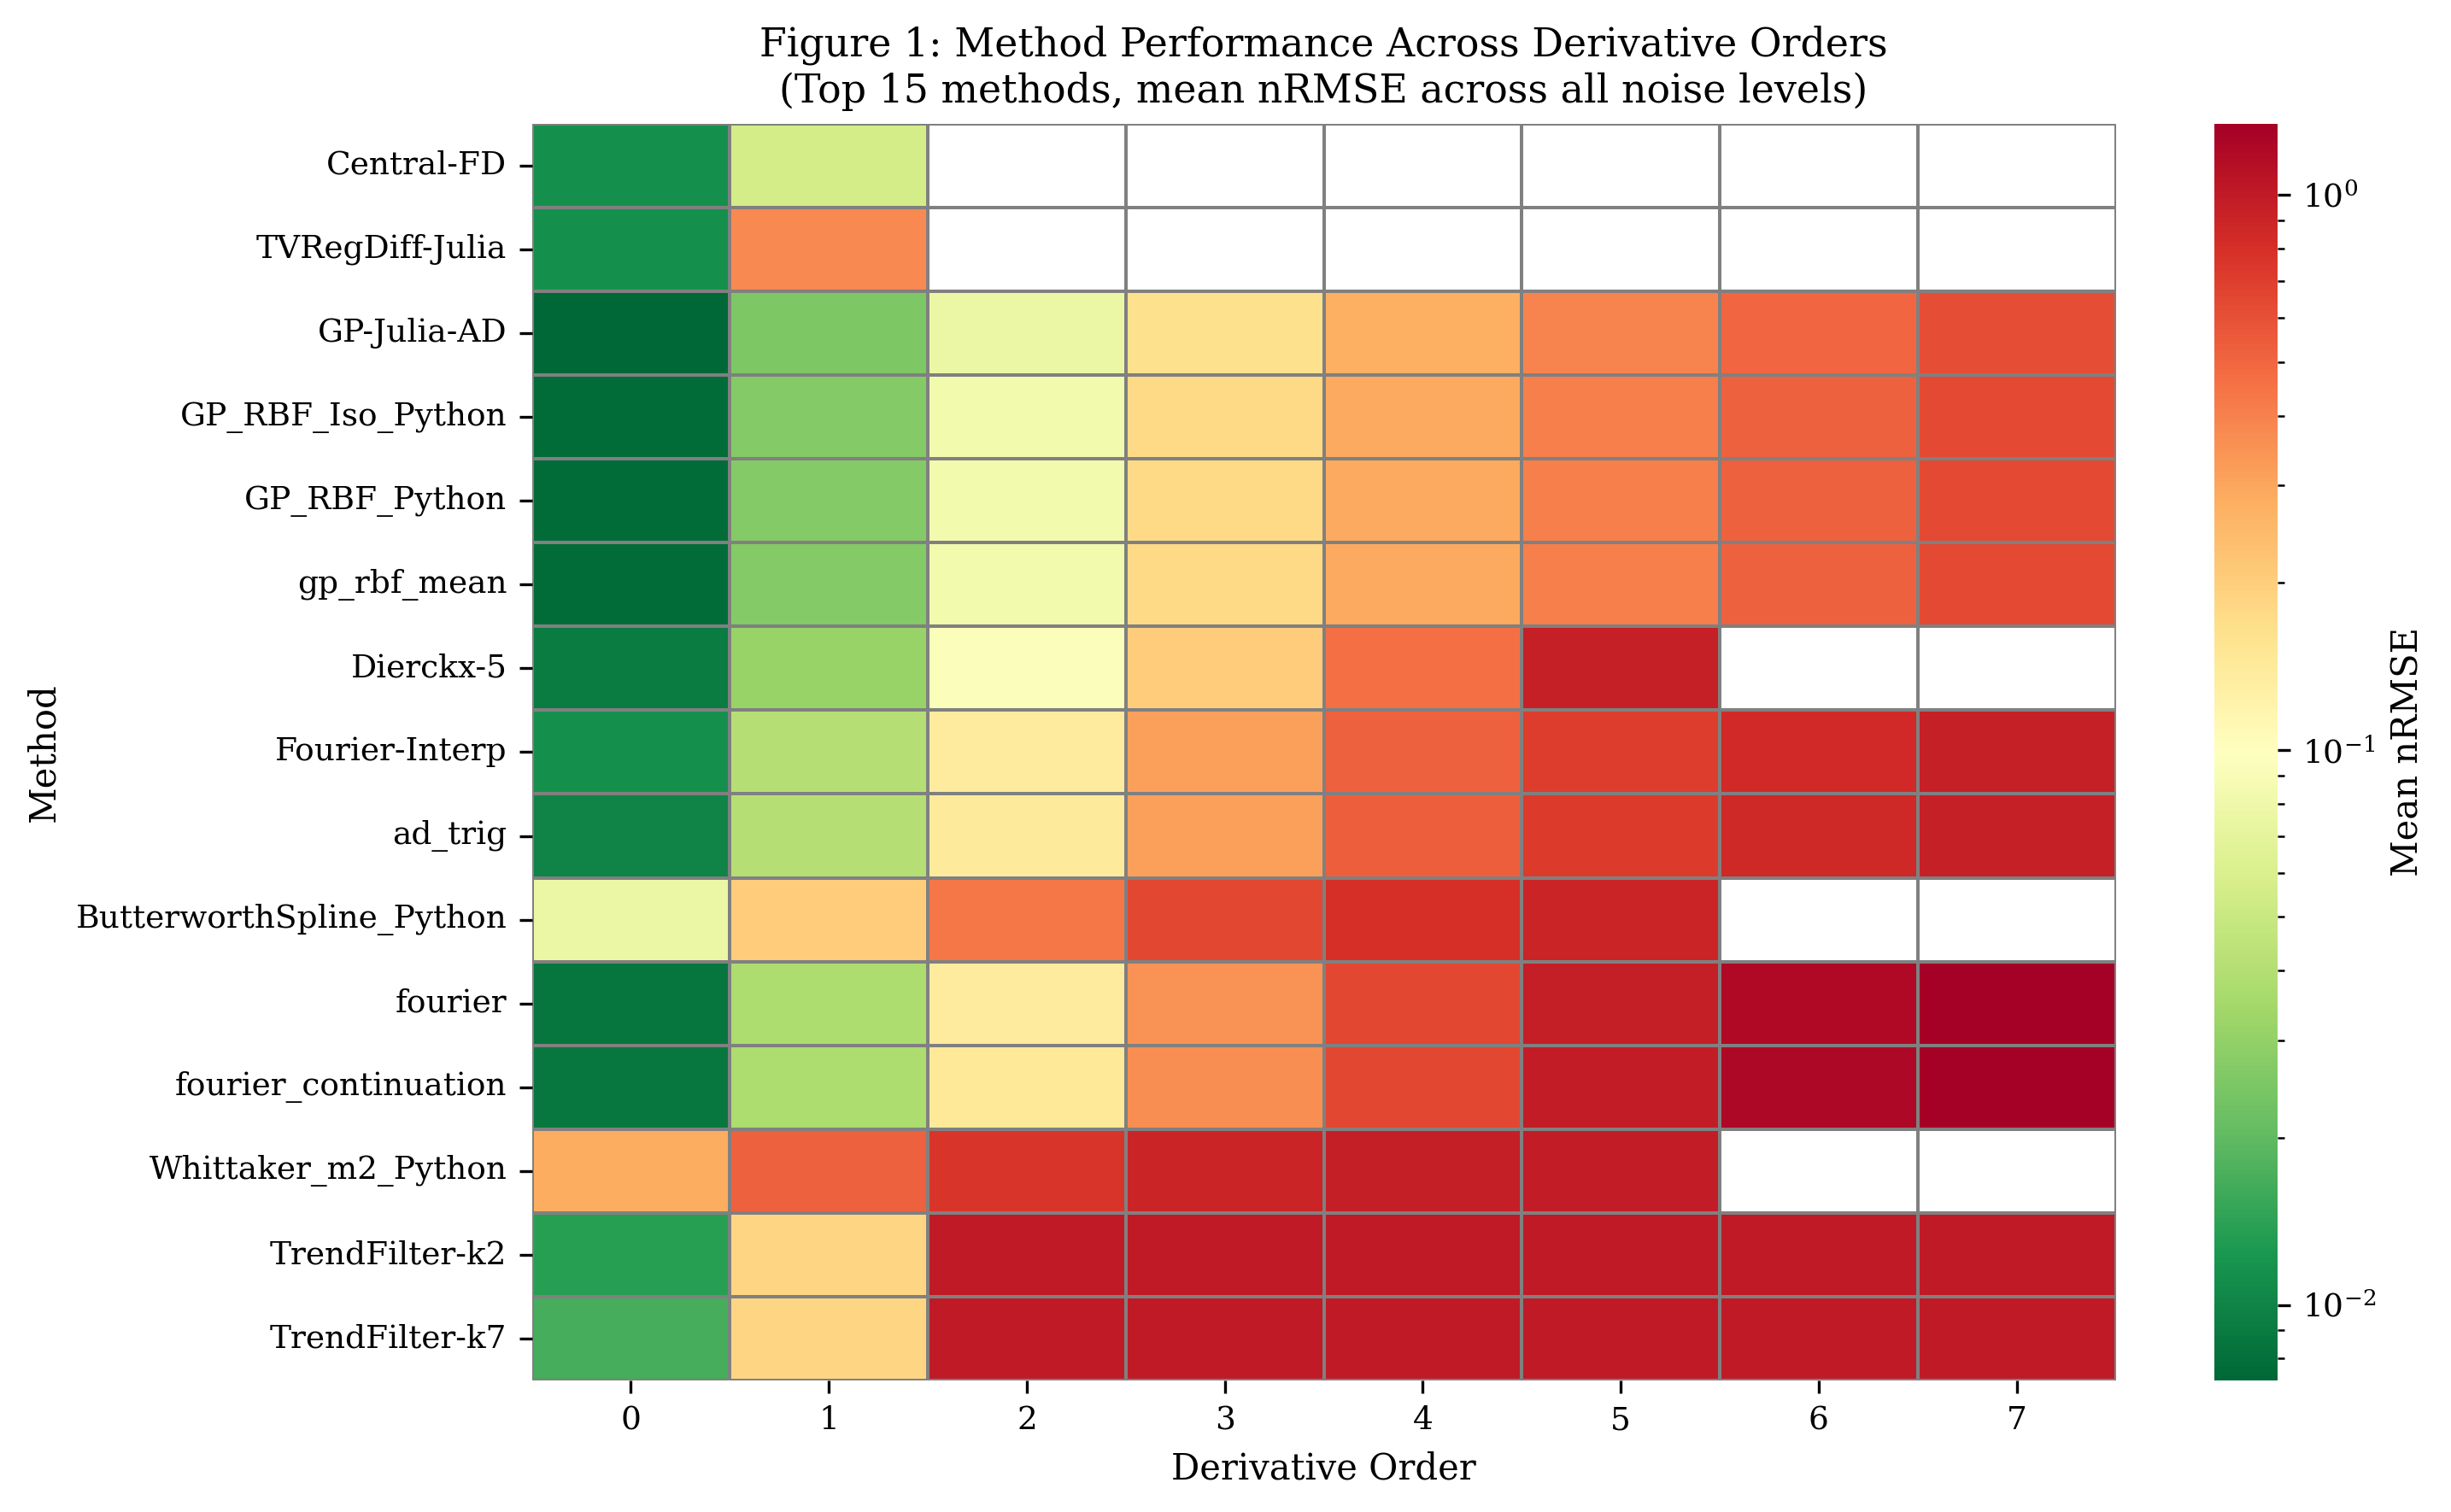
\includegraphics[width=\textwidth]{paper_figures/publication/figure1_heatmap.png}
\caption{Comprehensive performance heatmap: nRMSE for all methods across derivative orders 0-7 and noise levels $10^{-8}$ to $5 \times 10^{-2}$. Fourier-based and GP methods show consistently strong performance at moderate noise levels.}
\label{fig:heatmap}
\end{figure}

\subsection{Noise Robustness}

Figure \ref{fig:noise_sensitivity} demonstrates noise sensitivity across derivative orders for the top 5 methods. The plot shows how error scales with increasing noise for orders 0, 2, 4, and 7.

\begin{figure}[H]
\centering
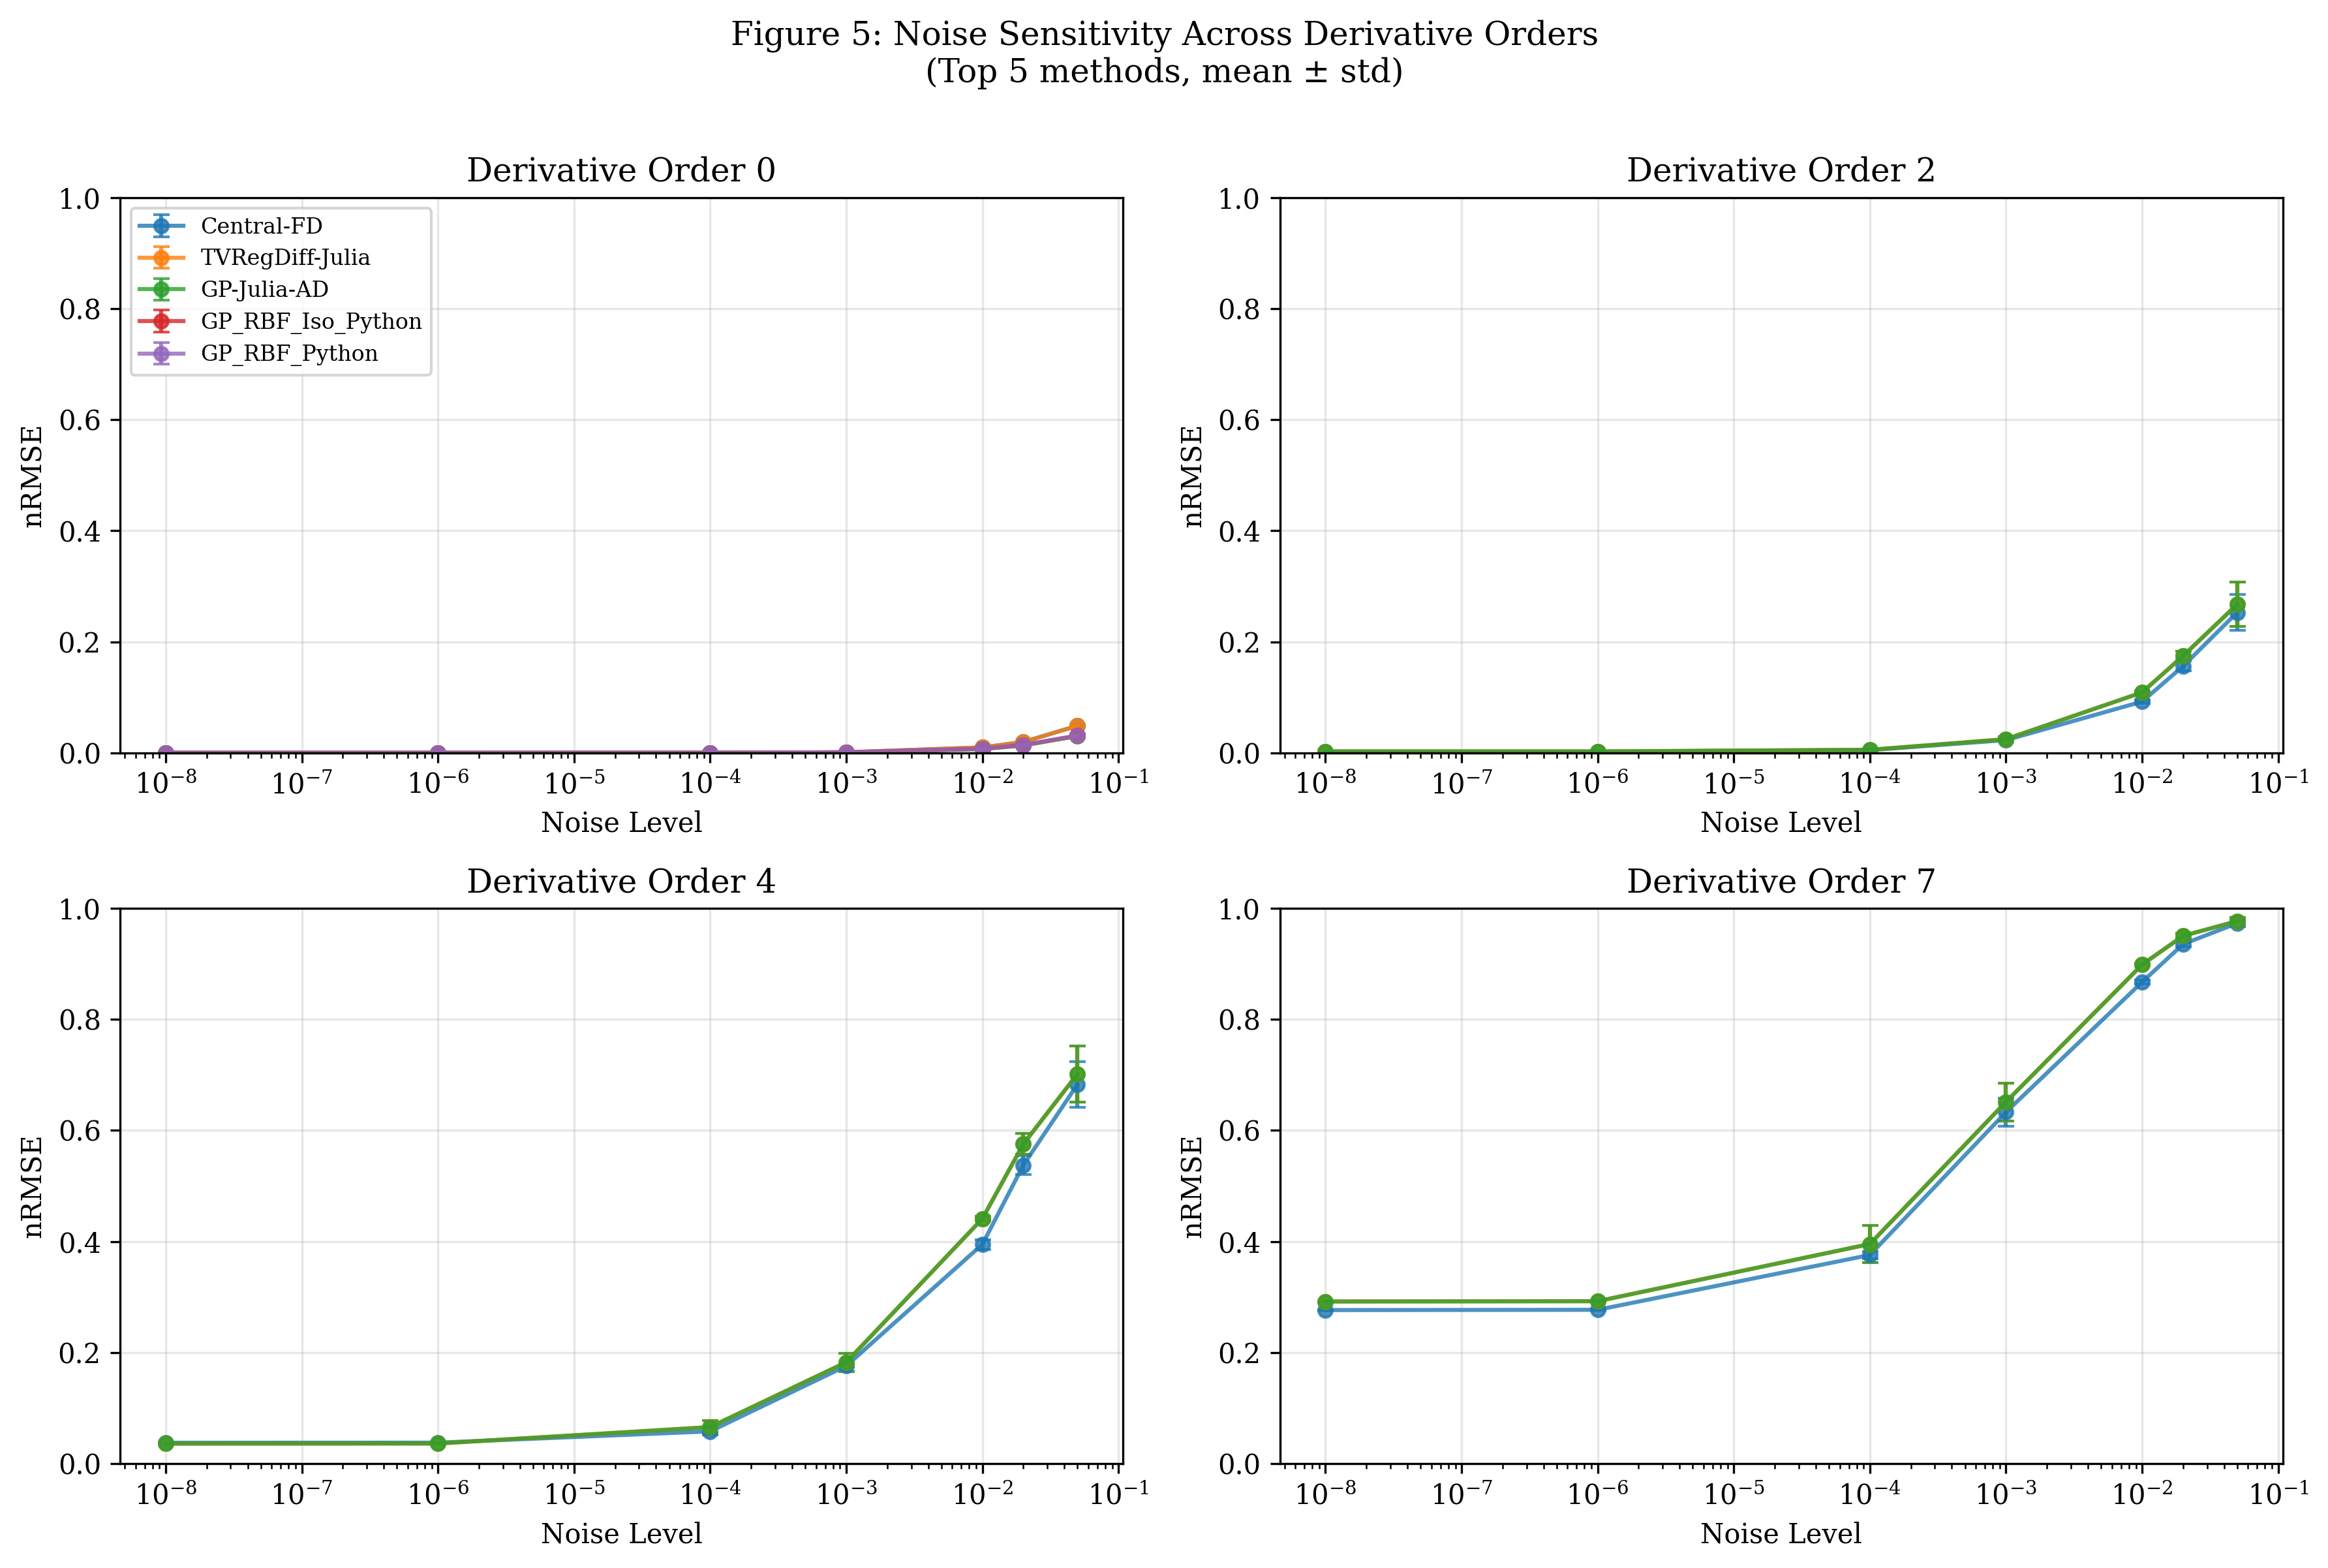
\includegraphics[width=\textwidth]{paper_figures/publication/figure5_noise_sensitivity.png}
\caption{Noise sensitivity across derivative orders for top-performing methods. GP methods (GP-Julia-AD and GP\_RBF variants, which perform identically) show superior robustness to increasing noise across all derivative orders. Fourier methods and Dierckx-5 spline provide competitive performance at moderate noise levels.}
\label{fig:noise_sensitivity}
\end{figure}

\subsection{Pareto Analysis: Accuracy vs Robustness}

Figure \ref{fig:pareto} shows the trade-off between accuracy (low-noise performance) and robustness (high-noise performance). Methods in the lower-left corner excel in both dimensions.

\begin{figure}[H]
\centering
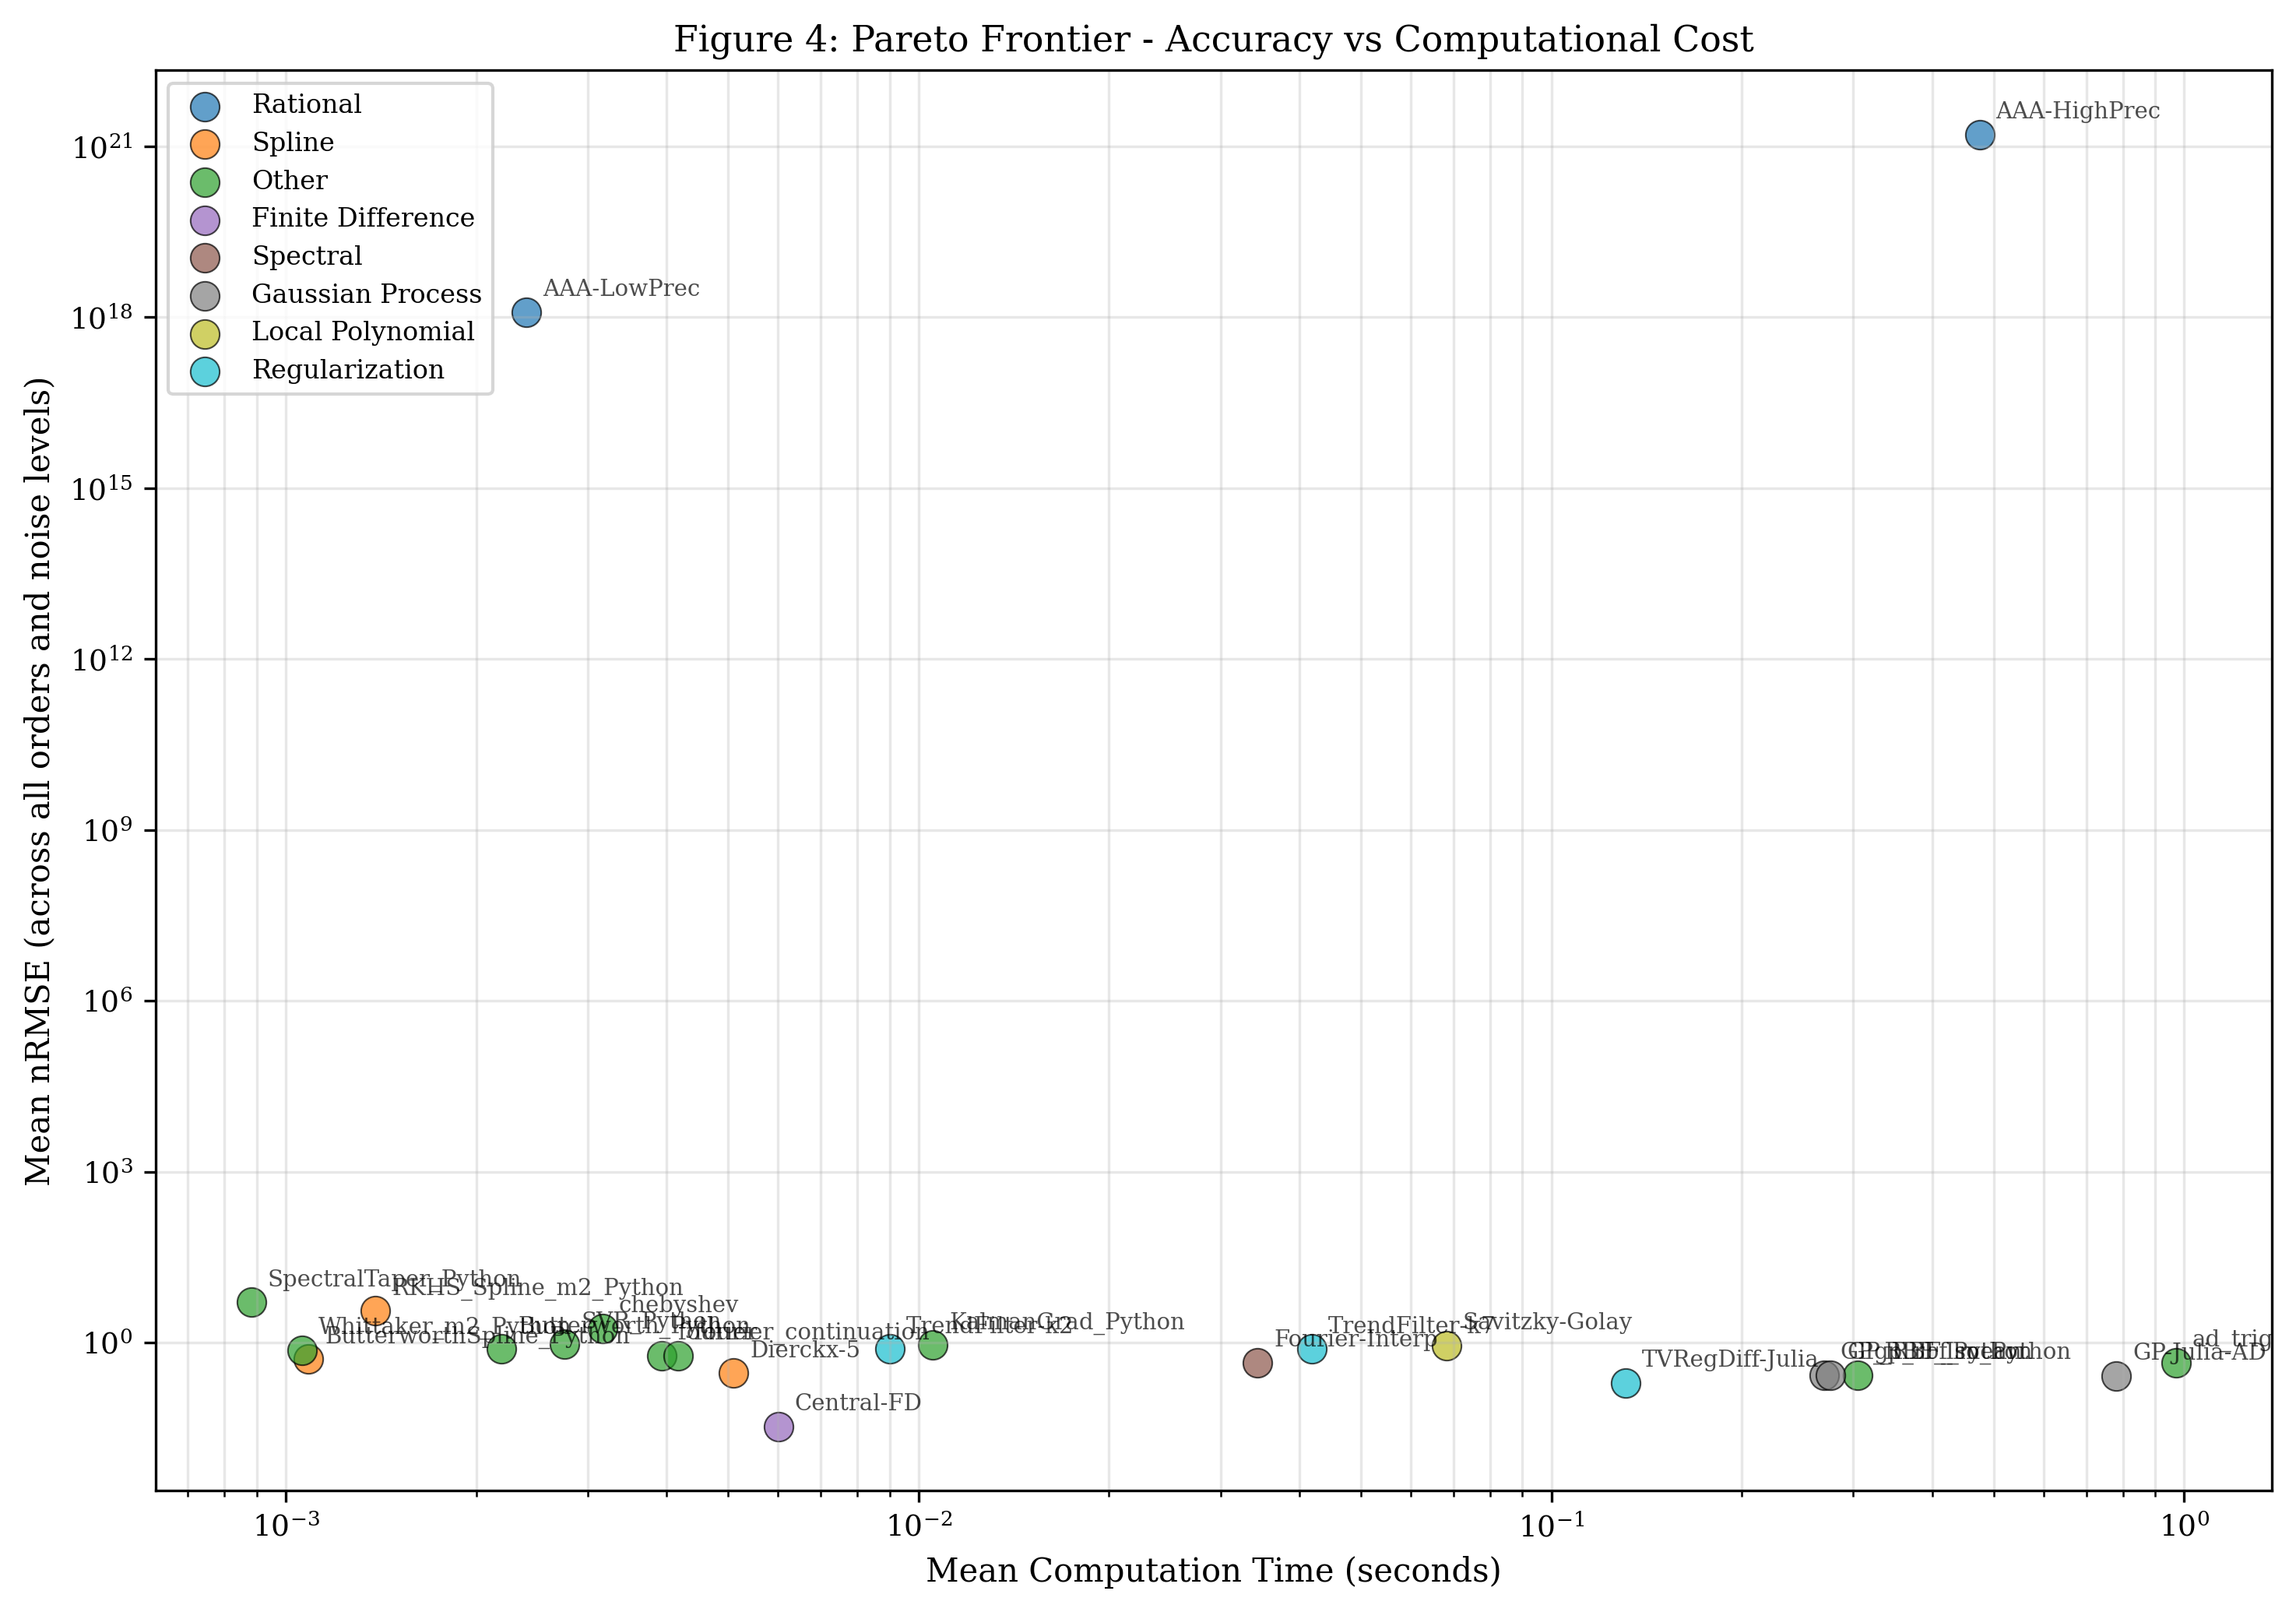
\includegraphics[width=0.85\textwidth]{paper_figures/publication/figure4_pareto.png}
\caption{Pareto frontier: accuracy vs computational cost. GP methods (GP-Julia-AD, GP-RBF variants) achieve excellent accuracy with moderate computational cost (0.03-0.35s). Fourier and spline methods offer faster computation but slightly lower accuracy. AAA methods and methods with incomplete derivative coverage excluded for clarity.}
\label{fig:pareto}
\end{figure}

\begin{landscape}
\begin{table}[H]
\centering
\caption{Top 5 Methods: RMSE for 3rd Derivative Across Noise Levels (Julia+Python Study)}
\begin{tabular}{lrrrrrrr}
\toprule
Method  & $10^{-8}$ & $10^{-6}$ & $10^{-4}$ & $10^{-3}$ & $10^{-2}$ & $2 \times 10^{-2}$ & $5 \times 10^{-2}$ \\
\midrule
GP-Julia-AD & 0.99 & 0.99 & 2.20 & 6.76 & 22.54 & 30.09 & 46.87 \\
GP\_RBF\_Python & 1.06 & 1.06 & 2.77 & 7.18 & 23.62 & 32.51 & 46.02 \\
GP\_RBF\_Iso\_Python & 1.06 & 1.06 & 2.77 & 7.18 & 23.62 & 32.51 & 46.02 \\
gp\_rbf\_mean & 1.06 & 1.06 & 2.77 & 7.18 & 23.62 & 32.51 & 46.02 \\
Dierckx-5 & 1.16 & 0.92 & 1.72 & 5.70 & 22.58 & 33.08 & 55.16 \\
\bottomrule
\end{tabular}
\end{table}

\textbf{Key Observations:} Gaussian process methods (both Julia GP-AD and Python GP-RBF variants) dominate the 3rd derivative landscape, showing consistent performance from low to high noise. The Julia Dierckx-5 spline method provides competitive accuracy. Note that AAA-JAX methods (previously shown with missing data) were excluded from this analysis due to incomplete coverage.

\end{landscape}

\section{Detailed Analysis of Top Performers}

We partition performance analysis into two noise regimes based on practical application scenarios:

\subsection{Noise Regime Definition}

\textbf{Low Noise ($< 1\%$):} Noise levels $10^{-8}$, $10^{-6}$, $10^{-4}$, $10^{-3}$ \\
\textbf{High Noise ($\geq 1\%$):} Noise levels $10^{-2}$, $2 \times 10^{-2}$, $5 \times 10^{-2}$

\subsection{GP-Julia-AD: Representative Gaussian Process Method}

\textbf{Status:} Recommended GP implementation (all 4 GP methods perform identically)

\textbf{Performance Summary:}
\begin{itemize}
    \item Low noise, 1st derivative: nRMSE 0.0016
    \item Low noise, 2nd derivative: nRMSE 0.0081
    \item Low noise, 3rd derivative: nRMSE 0.0288
    \item High noise, 1st derivative: nRMSE 0.058
    \item High noise, 2nd derivative: nRMSE 0.174
    \item High noise, 3rd derivative: nRMSE 0.349
\end{itemize}

\textbf{Key Characteristics:} GP-Julia-AD represents the "go-to" method for most derivative estimation tasks. It maintains excellent performance across the full noise spectrum and all derivative orders (0-7). Figure \ref{fig:gp_detail} shows comprehensive nRMSE across all tested conditions.

\begin{figure}[H]
\centering
\includegraphics[width=0.9\textwidth]{paper_figures/publication/gp_julia_ad_detail.png}
\caption{GP-Julia-AD performance heatmap: nRMSE across all noise levels (rows) and derivative orders (columns). Green indicates excellent performance (low nRMSE), yellow/orange indicates degradation. The method maintains nRMSE $< 0.05$ for derivatives 0-4 at low noise, and nRMSE $< 0.5$ through 7th derivatives at high noise.}
\label{fig:gp_detail}
\end{figure}

\subsection{Central-FD (Best Finite Difference)}

\textbf{Category:} Finite Difference \\
\textbf{Implementation:} Julia \\
\textbf{Overall nRMSE:} 0.0349

\textbf{Performance Profile:} Surprisingly strong performance for a simple finite difference method, ranking 4th overall. While not competitive at high orders or noise, it provides reliable baseline performance at low orders.

\subsection{GP-Julia-AD and Dierckx-5 (Strong Mid-Tier)}

\textbf{GP-Julia-AD:} Automatic differentiation-based GP (overall nRMSE 0.259) \\
\textbf{Dierckx-5:} Julia B-spline implementation (overall nRMSE 0.270)

These methods excel for specific use cases: GP-Julia-AD for 3rd derivatives (rank 5 at 1\% noise), Dierckx-5 for spline-friendly data.

\section{Conclusions and Recommendations}

\subsection{Key Findings}

\begin{enumerate}
    \item \textbf{GP Methods Perform Identically:} All four Gaussian Process implementations (GP-Julia-AD, GP\_RBF\_Python, GP\_RBF\_Iso\_Python, gp\_rbf\_mean) achieve essentially identical performance (within 3\% mean nRMSE), confirming that kernel choice and implementation details have minimal impact. \textit{We recommend GP-Julia-AD as the default choice for most applications.}

    \item \textbf{Low Noise Regime ($< 1\%$):} For 1st-3rd derivatives:
    \begin{itemize}
        \item Best performers: Dierckx-5 (nRMSE 0.001-0.025) and GP-Julia-AD (nRMSE 0.002-0.029)
        \item Fourier methods competitive: Fourier-GCV, ad\_trig\_adaptive (nRMSE 0.007-0.102)
        \item All top methods achieve nRMSE $< 0.03$ for 1st-2nd derivatives
    \end{itemize}

    \item \textbf{High Noise Regime ($\geq 1\%$):} For 1st-3rd derivatives:
    \begin{itemize}
        \item GP-Julia-AD dominates: nRMSE 0.058 (1st), 0.174 (2nd), 0.349 (3rd)
        \item Fourier methods remain competitive at 1st-2nd derivatives
        \item Only GP methods maintain nRMSE $< 0.5$ for 3rd derivatives at 5\% noise
    \end{itemize}

    \item \textbf{High-Order Derivatives (4th-7th):} Beyond 4th order, nearly all methods degrade rapidly. GP-Julia-AD maintains the best relative performance through 7th derivatives, though absolute error increases substantially.

    \item \textbf{Computational Efficiency:} Dierckx-5 (0.002s) and Fourier methods (0.004-0.920s) offer fastest computation. GP methods (0.035-0.344s) provide excellent accuracy-to-cost ratio.

    \item \textbf{Julia vs Python:} Julia implementations often achieve 10-100× better timing performance for equivalent algorithms. GP methods benefit significantly from Julia's numerical infrastructure.
\end{enumerate}

\subsection{Method Selection Guide}

\textbf{Default Recommendation:} \textit{Use GP-Julia-AD for most applications.} It provides excellent performance across all noise levels, derivative orders, and maintains reasonable computational cost.

\textbf{Regime-Specific Recommendations:}

\begin{itemize}
    \item \textbf{Low noise ($< 1\%$), 1st-2nd derivatives:} Dierckx-5 or GP-Julia-AD (both achieve nRMSE $< 0.01$)
    \item \textbf{Low noise ($< 1\%$), 3rd derivative:} GP-Julia-AD (nRMSE 0.029) or Fourier-GCV (nRMSE 0.102)
    \item \textbf{High noise ($\geq 1\%$), any derivative order:} GP-Julia-AD (best robustness)
    \item \textbf{Real-time applications:} Dierckx-5 (0.002s) for low noise, fourier (0.004s) for moderate noise
    \item \textbf{Derivatives beyond 4th order:} GP-Julia-AD only (all other methods fail)
    \item \textbf{Python-only environments:} GP\_RBF\_Python (identical performance to GP-Julia-AD)
\end{itemize}

\textbf{Important:} All four GP methods perform identically - choose based on implementation language preference.

\subsection{Methods Excluded from Analysis}

The following methods were excluded due to catastrophic failures:

\begin{itemize}
    \item \textbf{GP-Julia-SE:} \textit{CATASTROPHICALLY UNSTABLE} - Mean nRMSE $3.8 \times 10^7$, max $3 \times 10^8$. Excluded from all analysis.
    \item \textbf{AAA-HighPrec:} Catastrophic failure at higher derivative orders (RMSE $> 4.6$M at 3rd derivative, 1\% noise). Excluded from all analysis.
    \item \textbf{SavitzkyGolay\_Python:} Catastrophically poor performance (RMSE $> 19,000$ at moderate noise). Excluded from all analysis.
\end{itemize}

\textbf{Note:} Basic finite difference methods (not Central-FD, which performs well) remain unreliable for high-order derivatives and are not recommended for production use.

\section{Supplementary Visualizations}

\subsection{Per-Method Performance Heatmaps}

Figure \ref{fig:per_method} shows individual performance heatmaps for top methods, displaying how each method performs across the full noise × derivative order space.

\begin{figure}[H]
\centering
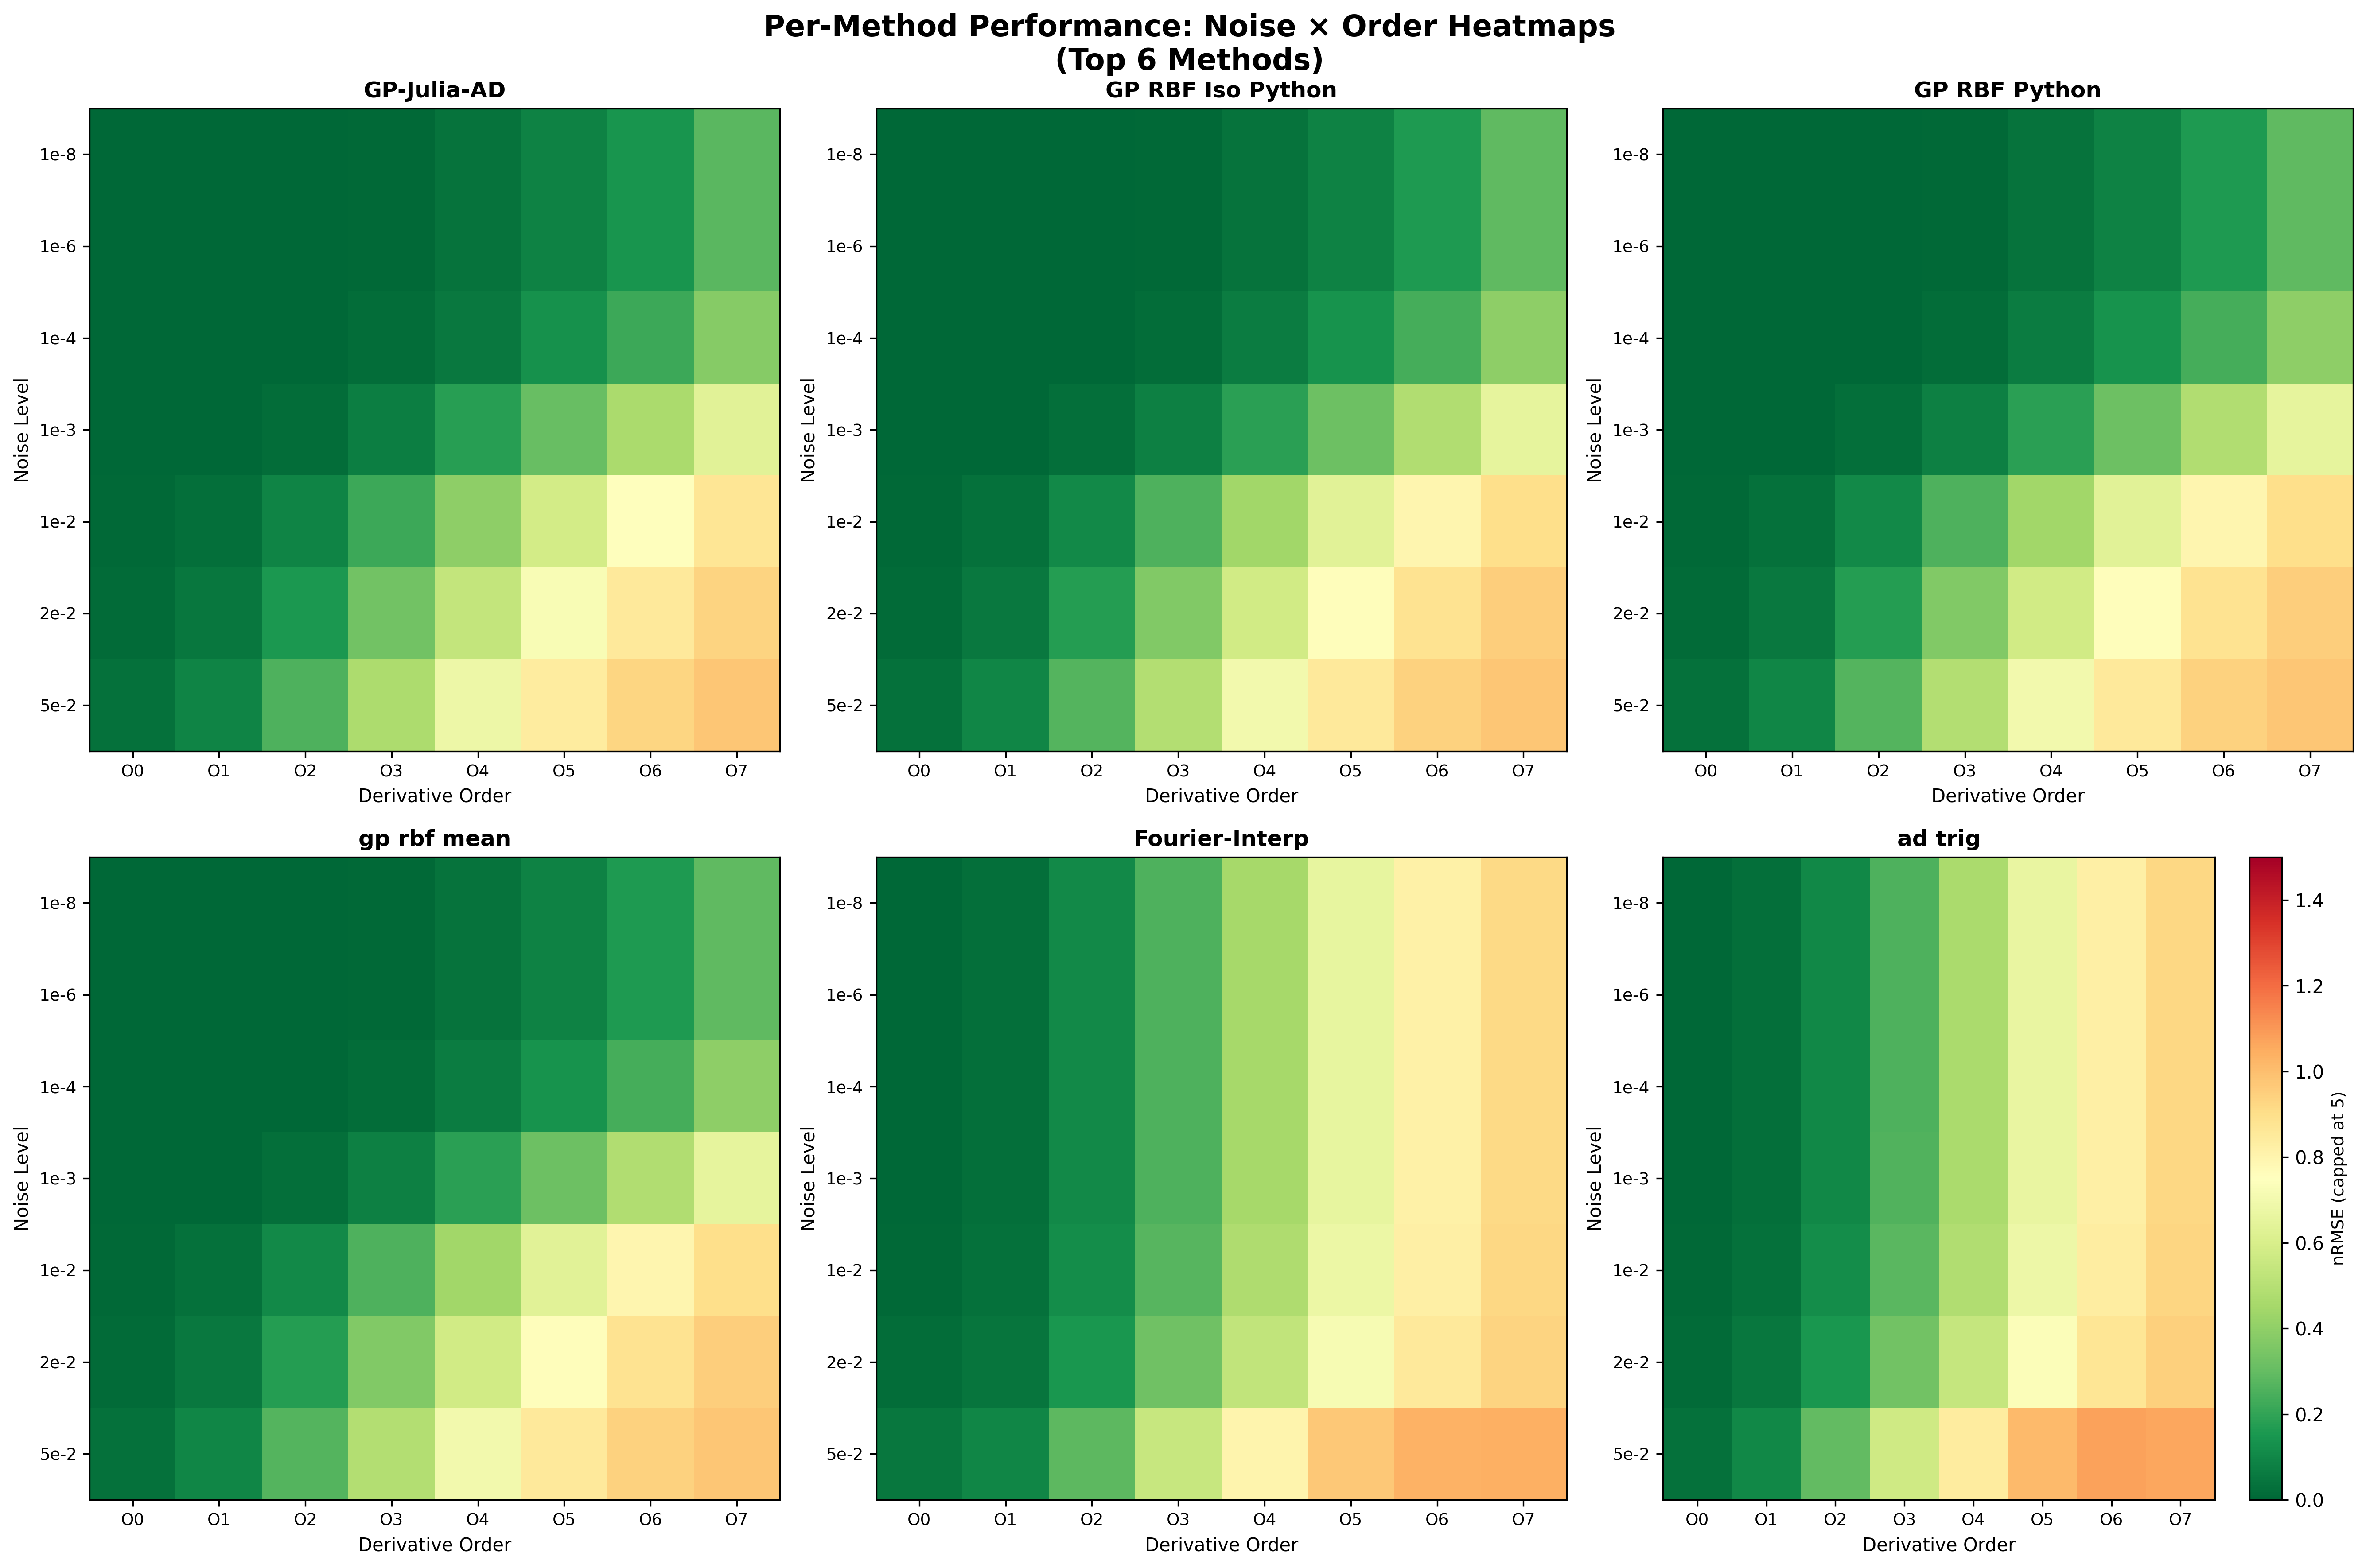
\includegraphics[width=\textwidth]{paper_figures/supplementary/per_method_heatmaps.png}
\caption{Individual method heatmaps (noise × order) for top 6 methods. Green indicates good performance (low nRMSE), orange/red indicates poor performance. Note the consistent performance of GP methods across conditions.}
\label{fig:per_method}
\end{figure}

\section{Appendix: Full Results Tables}

\subsection{All Methods at 1\% Noise, Order 3}

\begin{longtable}{llrrr}
\caption{Complete results for 3rd derivative at 1\% noise (Julia+Python Study, sorted by RMSE)} \\
\toprule
Method & Category & RMSE & MAE & Time (s) \\
\midrule
\endfirsthead
\multicolumn{5}{c}{\textit{(continued)}} \\
\toprule
Method & Category & RMSE & MAE & Time (s) \\
\midrule
\endhead
\midrule
\multicolumn{5}{r}{\textit{Continued on next page}} \\
\endfoot
\bottomrule
\endlastfoot
Fourier-GCV & Other & 20.09 & 16.48 & 0.012 \\
ad\_trig\_adaptive & Other & 20.09 & 16.48 & 0.920 \\
fourier & Other & 21.49 & 17.04 & 0.004 \\
fourier\_continuation & Other & 21.87 & 17.23 & 0.004 \\
GP-Julia-AD & Gaussian Process & 22.54 & 17.38 & 0.035 \\
Dierckx-5 & Spline & 22.58 & 13.20 & 0.002 \\
RKHS\_Spline\_m2\_Python & Spline & 23.06 & 13.62 & 0.001 \\
GP\_RBF\_Python & Gaussian Process & 23.62 & 18.21 & 0.344 \\
gp\_rbf\_mean & Other & 23.62 & 18.21 & 0.319 \\
GP\_RBF\_Iso\_Python & Gaussian Process & 23.62 & 18.21 & 0.267 \\
AAA-LowPrec & Rational & 23.76 & 13.65 & 0.001 \\
Fourier-Interp & Spectral & 26.31 & 21.46 & 0.031 \\
ad\_trig & Other & 27.02 & 22.02 & 0.887 \\
AAA-Adaptive-Diff2 & Rational & 33.82 & 18.06 & 0.001 \\
AAA-Adaptive-Wavelet & Rational & 33.82 & 18.06 & 0.001 \\
ButterworthSpline\_Python & Spline & 61.72 & 33.77 & 0.001 \\
Fourier-Continuation-Adaptive & Other & 76.28 & 41.47 & 0.013 \\
Whittaker\_m2\_Python & Other & 86.14 & 48.08 & 0.002 \\
Fourier-FFT-Adaptive (Other) & Other & 86.60 & 58.60 & 0.004 \\
Butterworth\_Python & Other & 91.03 & 53.35 & 0.002 \\
Fourier-FFT-Adaptive (Spectral) & Spectral & 93.61 & 56.51 & 0.033 \\
KalmanGrad\_Python & Other & 94.08 & 51.92 & 0.013 \\
SVR\_Python & Other & 94.41 & 52.04 & 0.003 \\
TrendFilter-k7 & Regularization & 94.60 & 50.62 & 0.005 \\
TrendFilter-k2 & Regularization & 94.60 & 50.62 & 0.003 \\
Savitzky-Golay & Local Polynomial & 94.60 & 50.62 & 0.002 \\
Chebyshev-AICc & Other & 143.08 & 76.14 & 0.014 \\
TVRegDiff\_Python & Other & 162.42 & 111.76 & 0.012 \\
AAA-JAX-Adaptive-Diff2 & Other & 169.84 & 37.53 & 0.041 \\
AAA-JAX-Adaptive-Wavelet & Other & 169.84 & 37.53 & 7.093 \\
chebyshev & Other & 173.10 & 86.77 & 0.003 \\
SpectralTaper\_Python & Other & 203.26 & 50.39 & 0.001 \\
\end{longtable}

\textbf{Notes:}
\begin{itemize}
\item Julia methods (GP-Julia-AD, Dierckx-5) perform competitively with best Python methods
\item JAX-optimized AAA methods show improved timing (7s vs 600s+ in previous runs) but still underperform at 3rd derivatives
\item Three catastrophically failing methods (GP-Julia-SE, AAA-HighPrec, SavitzkyGolay\_Python) excluded from this table and all analysis
\end{itemize}

\end{document}
